\documentclass[11pt,pdftex,portrait,letterpaper]{article}
\usepackage[hdivide={1in,*,1in},
            vdivide={1in,*,1in},
%            showframe
            ]{geometry}

\usepackage{graphicx}
\usepackage{longtable}
\usepackage{acronym}
\usepackage{verbatim}
\usepackage{subfigure}
\usepackage{fancyhdr}
\pagestyle{fancy}
\usepackage{listings}
\usepackage{color}
\usepackage{lastpage}

% Default margins are too wide all the way around. Reset them here
\setlength{\topmargin}{-.5in}
\setlength{\textheight}{9in}
\setlength{\oddsidemargin}{.125in}
\setlength{\textwidth}{6.25in}

\lhead{ELEC 222}
\chead{}
\rhead{\thepage\ of \pageref{LastPage}}
%\lfoot{\hline}
\lfoot{}
\cfoot{\small{University of Nebraska - Lincoln Department of Electrical Engineering}}
\rfoot{}
\renewcommand{\footrulewidth}{0.5pt}


% Modify parameters of Listings
\lstset{ 
language=C,
basicstyle=\scriptsize,
numbers=left,
numberstyle=\footnotesize,
stepnumber=1,
numbersep=10pt,
backgroundcolor=\color{white},
frame=single,
captionpos=b,
breaklines=true,
breakatwhitespace=false
}

\begin{document}

\vspace*{30ex}
\begin{center}

\textbf{Project 03 - DSP/BIOS based FIR }\\

\vspace{4ex}
Introduction to Embedded Systems - University of Nebraska \\

\vspace{4ex}
Zach Swanson\\

\end{center}


\pagebreak
\tableofcontents
%\pagebreak
%\listoffigures
%\addcontentsline{toc}{section}{{\bf List of Figures}}
\pagebreak


\section{Introduction}

The purpose of this project was to introduce the Texas Instruments (TI) real-time operating system BIOS using the TI ezDSP5535 development board (ezDSP). The project required the use of hardware interrupt (HWI) threads, software interrupt (SWI) threads, and idle (IDL) threads. The goal of the project was to receive, filter and retransmit audio samples using HWIs and SWIs. Additional components to change between a low-pass (bass) and high-pass (treble) filter and to transmit a one kHz tone were included to employ the IDL threads. The project built on previous projects by requiring the use of myNCO and myFIR functions designed in Projects 1 and 2, respectively.
 
\section{Project Description}

\subsection{Filter Design}

Two filters were implemented for this project, a low- and high-pass filter, with the intent of isolating bass tones with the low-pass filter and isolating treble tones with the high-pass filter. The design process was trial-and-error until filters were achieved that produced the distinct bass and treble sounds that were desired. 

The low-pass filter was designed with the following specifications: 

\begin{itemize}
\item Passband frequency: \textbf{350 Hz}
\item Stopband frequency: \textbf{1310 Hz}
\item Passband ripple: \textbf{0.2 dB}
\item Stopband attenuation: \textbf{60 dB}
\item Order: \textbf{125}
\end{itemize}

The high-pass filter was designed with the following specifications:

\begin{itemize}
\item Passband frequency: \textbf{2100 Hz}
\item Stopband frequency: \textbf{1400 Hz}
\item Passband ripple: \textbf{0.2 dB}
\item Stopband attenuation: \textbf{60 dB}
\item Order: \textbf{124}
\end{itemize}

The frequency response of both filters is shown in Figure \ref{f:fig1}.

\begin{figure}[h]
\centering
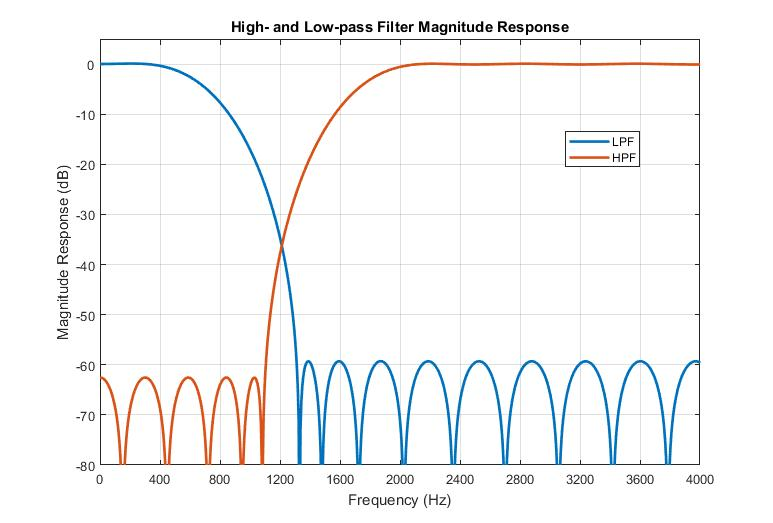
\includegraphics[width=0.8\textwidth]{./magRsp}
\caption{Magnitude response of low- and high-pass filters}
\label{f:fig1}
\end{figure}

\subsection{Program Description}

TI provides an easy-to-use GCONF tool to configure the BIOS scheduler, which was used to establish the threads that were used for this project. To progress through the project incrementally the HWIs were setup and tested, the SWI was incorporated and finally the IDL threads were included. HWI 14 and 15 were used for I2S transmit (tx) and I2S receive (rx) with function handles\_ HWI\_I2S\_Tx and \_HWI\_I2S\_Rx, respectively. Two SWI threads with function handles \_SWIPingFunc and \_SWIPongFunc and equal priority were defined using GCONF. Lastly, the GCONF tool was used establish two IDL threads with function handles \_monitorSW1 and \_monitorSW2.

After establishing the threads using GCONF, the HWI threads were enabled in main and once the program exited main it launched the DSP/BIOS scheduler, which managed all the threads. The scheduler ensures that threads run in the correct order based on priority. In general, the priority level of thread types is HWI, SWI, IDL, in descending order.

\subsection{HWI\_I2S\_Rx}

Listing \ref{l:programa} shows the code for the HWI thread that handled I2S reception . It was assumed that the right and left samples were the same; therefore, the right sample was read and disregarded and the left sample was stored into a double buffer. The double buffer was 96 elements and was broken into two 48 element buffers, ping and pong. The purpose of the double buffer was that once ping was full its elements could be filtered while new data was loaded into pong. Otherwise, if a single buffer was used, then data may be lost during the process of filtering. The double buffer is reflected in the code. New data is stored in the double buffer rxPingPong until 48 samples have been received; then, the HWI posts the software interrupt SWIPing which handles filtering of the ping buffer. While SWIPingFunc filters the samples the HWI continues to place new samples into pong, i.e. the latter half of rxPingPong. Samples are stored until 48 more have been received, and the HWI posts a second SWI to filter the pong samples.

\begin{lstlisting}[caption={I2S receive HWI thread}, label=l:programa]
void HWI_I2S_Rx(void)
{
	volatile int16_t temp;
	temp = hI2s->hwRegs->I2SRXRT1;
	rxPingPong[rxIndex++] = hI2s->hwRegs->I2SRXLT1;

	if (rxIndex == 48)		//Have 48 samples been collected
	{
		/* Ping is full */
		SWI_post(&SWIPing);
	}
	if (rxIndex == 96)
	{
		/* Pong is full */
		SWI_post(&SWIPong);
		rxIndex = 0;
	}
}
\end{lstlisting}

\subsection{HWI\_I2S\_Tx}

Listing \ref{l:programb} shows the code for the HWI thread that handled I2S transmission. This thread simply writes the filtered samples to the I2S, checks to see if the end of the array has been reached and resets back to the beginning of the transmit array if it has.

\begin{lstlisting}[caption={I2S transmit HWI thread}, label=l:programb]
void HWI_I2S_Tx(void)
{
	hI2s->hwRegs->I2STXLT1 = txPingPong[txIndex];
	hI2s->hwRegs->I2STXRT1 = txPingPong[txIndex++];

	if (txIndex == 96)		//Have 96 samples been transmitted?
	{
		txIndex = 0;
	}
}
\end{lstlisting}

\subsection{SWI\_PingFunc and SWI\_PongFunc}

Listing \ref{l:programc} shows the code for the SWI thread that filtered samples in the ping array. The SWI thread for the filtering pong was not included because it was very similar. The SWI calls the myfir function designed in project 2, which used a delayline approach for implementing a FIR filter. The function took the ping array (i.e. samples 0-47 of rxPingPong), sampled all 48 samples and stored in txPingPong. To be able to switch between filters, a pointer was used to point to either the array of low-pass or high-pass coefficients and another pointer pointed to the filters' corresponding delayline array.

The ping and pong threads only ran when they had been posted by the rx HWI thread.

\begin{lstlisting}[caption={Ping filter SWI thread}, label=l:programc]
void SWIPingFunc(void)
{
	myfir(&rxPingPong[0], filterPtr, &txPingPong[0], delayLinePtr, NX, myNH);
}
\end{lstlisting}

\subsection{montiorSW1}

Listing \ref{l:programd} shows the code for the IDL thread that monitored for switch one strokes. When the thread detected a switch stroke, it disabled all SWIs and HWI ensure that a one kHz tone was played for one second without being interrupted and to prevent other samples from being transmitted with tone. The tone was generated using myNCO from project 1. Once the tone played, both delaylines were cleared and the double buffer indexes were reset before enabling SWIs and restoring the HWIs to their previous state. 

This thread would run when the HWIs and SWIs were not running and occurred sequentially with the other IDL thread.

\begin{lstlisting}[caption={IDL thread for monitoring switch one strokes and playing a tone}, label=l:programd]
void monitorSW1(void)
{
	/* Check SW1 */
	if(EZDSP5535_SAR_getKey( ) == SW1) // Is SW1 pressed?
	{
		if(sw1State)              // Was previous state not pressed?
		{
			int16_t msec, sample;

			/* Disable SWIs and HWIs -- store HWI state */
			SWI_disable( );
			Uns oldState1 = HWI_disable( );

			/* nested for loop to play 1 kHz tone for 1 sec */
			for ( msec = 0 ; msec < 1000 ; msec++ )
			{
				for ( sample = 0 ; sample < 48 ; sample++ )
				{
					/* call myNCO to get 1 kHz tone sample */
					int16_t temp = (myNCO( 1000 ) >> 5);

	                			/* Write 16-bit left channel Data */
	              			EZDSP5535_I2S_writeLeft( temp );

					/* Write 16-bit right channel Data */
					EZDSP5535_I2S_writeRight( temp );
				}
			}
			/* clear phase accumulator */
			clearPA( );

			/* clear both delayLines and reset rx and tx indices */
			memset(delayLineLPF, 0, sizeof(delayLineLPF));
			memset(delayLineHPF, 0, sizeof(delayLineHPF));
			rxIndex = 0;
			txIndex = 0;

			/* restore HWIs to previous state and enable SWIs */
			HWI_restore( oldState1 );
			SWI_enable( );

			sw1State = 0;     // Set state to 0 to allow only single press
		}
	} else                      // SW1 not pressed
	{
		sw1State = 1;         // Set state to 1 to allow timer change
	}
}
\end{lstlisting}

\subsection{monitorSW2}

Listing \ref{l:programe} shows the code for the IDL thread that monitored for switch two strokes. When the thread detected a switch stroke, it checked to see if the low-pass or high-pass filter was being used and proceeded to implement the alternate filter. As mentioned, two delaylines were used because the filters differed in length, which required different length delaylines. When switching filters the new filter's delay line was cleared. This generated a brief disturbance in the audio that was noticed if focused on trying to hear the sound. It was determined that the minor disturbance was a lower cost than the noise generated by having a single delayline or the cycles required to dump one delayline into another. Additionally, it provided an easier means of implementation. To make switching between filter and delayline arrays easier, pointer variables were used to simply point to the desired arrays.

\begin{lstlisting}[caption={IDL thread for monitoring switch two strokes and changing filters}, label=l:programe]
void monitorSW2(void)
{
	/* Check SW2 */
	if(EZDSP5535_SAR_getKey( ) == SW2) // Is SW2 pressed?
	{
		if(sw2State)          // Was previous state not pressed?
		{
			if(filtState)		//Was previous state High-pass?
			{
				/* Clear Low-pass delayLine */
				memset(delayLineLPF, 0, sizeof(delayLineLPF));

				/* Point filter pointer to myLPF */
				filterPtr = &myLPF[0];

				/* Point delay line pointer to delayLineLPF */
				delayLinePtr = &delayLineLPF[0];

				/* Set myNH to number of low-pass coefficients */
				myNH = LPF_NH;

				/* Set filtState to low-pass */
				filtState = 0;
			} else				//Was previous state low-pass
			{
				/* Clear high-pass delay line */
				memset(delayLineHPF, 0, sizeof(delayLineHPF));

				/* Point filter pointer to myHPF */
				filterPtr = &myHPF[0];

				/* Point delayline pointer to delayLineHPF */
				delayLinePtr = &delayLineHPF[0];

				/* Set my NH to number of high-pass coefficients */
				myNH = HPF_NH;

				/* Set filtState to high-pass */
				filtState = 1;
			}
			sw2State = 0;     // Set state to 0 to allow only single press
		}
	} else                      // SW2 not pressed
	{
		sw2State = 1;         // Set state to 1 to allow tone change
	}
\end{lstlisting}

\section{Results}

\subsection{CPU Usage}

Both the rx and the tx HWIs required 16 cycles per sample. With a 100 MHz CPU and 48 kHz codec, 2,083 cycles per sample were available; hence, each HWI used 0.77 percent of the CPU time.

The SWIs required approximately 20,000 cycles per frame of samples. At 48 samples per frame, each sample required 417 cycles and the CPU load for the SWIs was 20 percent.

\subsection{Execution Graph}

To implement an execution graph, a LED was turned off when the BIOS scheduler entered a thread and was turned back on when it returned from the thread. Therefore, on a logic analyzer the line was pulled high when entering a thread and pushed low when exiting. The red LED was not used because the hardware pulled the line low enough to turn off the LED but did not pull it low enough to register as low on the logic analyzer. As a result, on three threads were monitored at a time. 

Figure \ref{f:fig2} shows an execution graph of the I2S rx HWI (top), both ping and pong SWIs (middle), and both IDL threads (bottom). The HWI and the SWI graphs were similar to what was expected. As the measurement shows, every 48 times the HWI occured another SWI was posted and the HWI continued to occur while the SWI was running. In reality, each time the tx or rx HWI occurred the SWI graph would go low since the HWIs would have higher priority. Such a graph was generated, but it was difficult to decipher the graph and the graph proivded was generated instead. It was interesting to observe the amount of time that it took each IDL thread to run. As the lowest priority thread type, the IDL was continually interrupted and took longer to execut as a result. It became obvious that if too many higher priority threads were running then the IDL thread may never be reached.

\begin{figure}[h]
\centering
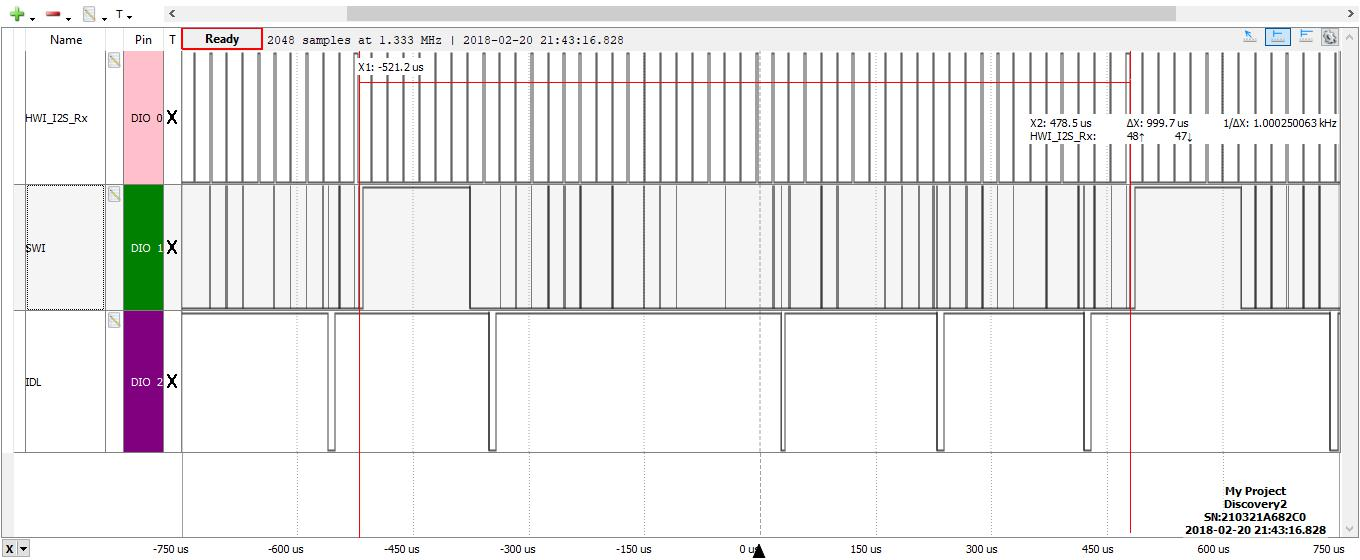
\includegraphics[width=0.8\textwidth]{./execution1}
\caption{Execution of I2S rx HWI, ping and pong SWI, and both IDL threads}
\label{f:fig2}
\end{figure}

Figure \ref{f:fig3} shows another execution graph with the I2S tx HWI (bottom) instead of the IDL threads. Note the measurement, which inidicates that the HWI is clocked at the codec sampling frequency of 48 kHz as expected. 

\begin{figure}[h]
\centering
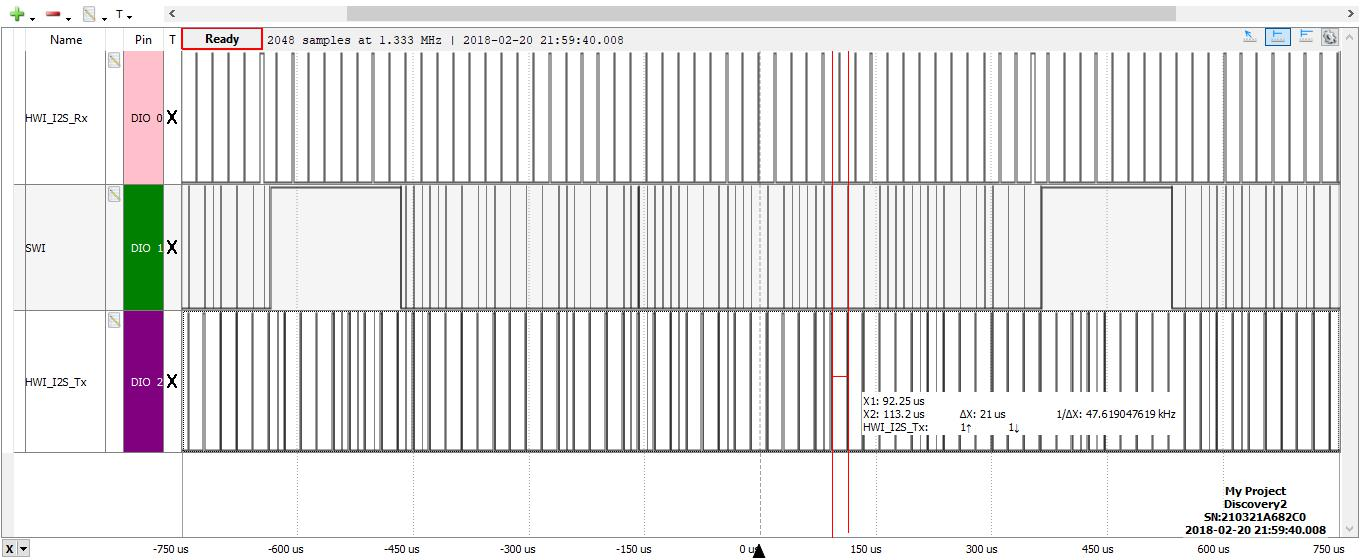
\includegraphics[width=0.8\textwidth]{./execution2}
\caption{Execution of I2S rx HWI, ping and pong SWI, and I2S tx HWI threads}
\label{f:fig3}
\end{figure}

Additionally, the time between the SWI thread going high and going low was measured to 168.7 microseconds. This time correspongs to a CPU load of 16.87 percent, which varied slightly from the aforementioned CPU load. 

\subsection{Demonstration}

The project demonstrated as expected, except for the function of the buttons. When pressing switch two, especially when pressing rapidly, the board would register the press as switch one and perform the wrong operation. After investigating the issue, it was discovered that the design of the switches is less than desireable. Switch one is connected by a 20 k$\Omega$ resistor to an ADC and switch two is connected by a 10 k$\Omega$ resistor to the same ADC. The ADC values for switch one and two are close enough that switch two will occassionally generate a value higher than the switch one value. Therefore, the problem could not be fixed by changing the threshold values and the issue pursued no further.

\section{Summary}

This project introduced and showed the significance of using real-time operating systems. After completing the project, I have ideas of trying to implement RTOSs in other projects where I believe the scheduling nature may be useful and appropriate.

\pagebreak

\section{Appendix}

\begin{lstlisting}[caption={main.c}, label=l:programx]
#include <std.h>

#include <log.h>

#include "hellocfg.h"
#include "ezdsp5535.h"
#include "ezdsp5535_led.h"
#include "ezdsp5535_sar.h"
#include "ezdsp5535_i2s.h"
#include "csl_i2s.h"
#include "stdint.h"
#include "aic3204.h"

extern CSL_I2sHandle   hI2s;
extern void audioProcessingInit(void);


void main(void)
{
    LOG_printf(&trace, "hello world!");

    /* Initialize BSL */
    EZDSP5535_init( );

    /* init LEDs and set to off*/
    EZDSP5535_LED_init( );
    EZDSP5535_LED_setall(0x0F);

    /* init dip switches */
    EZDSP5535_SAR_init( );

    // configure the Codec chip
    ConfigureAic3204();

    /* Initialize I2S */
    EZDSP5535_I2S_init();

    /* enable the interrupt with BIOS call */
    C55_enableInt(14); // reference technical manual, I2S2 tx interrupt
    C55_enableInt(15); // reference technical manual, I2S2 rx interrupt

    audioProcessingInit();

    // after main() exits the DSP/BIOS scheduler starts
}

\end{lstlisting}
\pagebreak

\begin{lstlisting}[caption={audioProcessing.c}, label=l:programxx]
/*
 *  Copyright 2010 by Texas Instruments Incorporated.
 *  All rights reserved. Property of Texas Instruments Incorporated.
 *  Restricted rights to use, duplicate or disclose this code are
 *  granted through contract.
 *
 */
/***************************************************************************/
/*                                                                         */
/*     H E L L O . C                                                       */
/*                                                                         */
/*     Basic LOG event operation from main.                                */
/*                                                                         */
/***************************************************************************/

#include <std.h>

#include <log.h>

#include "stdint.h"
#include "string.h"
#include "hellocfg.h"
#include "ezdsp5535.h"
#include "ezdsp5535_gpio.h"
#include "ezdsp5535_led.h"
#include "ezdsp5535_sar.h"
#include "ezdsp5535_i2s.h"
#include "csl_i2s.h"
#include "csl_gpio.h"
#include "aic3204.h"
#include "filters.h"

#define NX			48
#define BL_ONLY		0x0E
#define YL_ONLY		0x0D
#define RD_ONLY		0x0B
#define GR_ONLY		0x07
#define MIN(a,b) ( ((a) <  (b)) ? (a) : (b) )

extern CSL_I2sHandle   hI2s;
extern void myfir(const int16_t* input, const int16_t* filterCoeffs,
		int16_t* output, int16_t* delayLine, uint16_t  nx, uint16_t  nh);
extern int16_t myNCO(uint16_t f_tone);
extern void clearPA(void);

int16_t rxPingPong[96];
int16_t txPingPong[96];

int16_t delayLineLPF[NX + LPF_NH - 1];
int16_t delayLineHPF[NX + HPF_NH - 1];

int16_t rxIndex;
int16_t txIndex;

uint16_t sw1State  = 0;       	// SW1 state
uint16_t sw2State  = 0;       	// SW2 state
uint16_t filtState = 0;			// filter state

int16_t * filterPtr;
int16_t * delayLinePtr;
uint16_t myNH;

Uint16 idl = 0, swi = 0;

/*
 * audioProcessingInit
 *
 * @brief: 	Initialize arrays used for filtering and transmitting
 * 			and initialize array indices to 0.
 */
void audioProcessingInit(void)
{
	/* Initialize arrays as empty*/
	memset(txPingPong, 0, sizeof(txPingPong));
	memset(delayLineLPF, 0, sizeof(delayLineLPF));
	memset(delayLineHPF, 0, sizeof(delayLineHPF));

	/* Initially select low-pass filter */
	filterPtr = &myLPF[0];
	delayLinePtr = &delayLineLPF[0];
	myNH = LPF_NH;

	/* Initialize rx and tx indices to 0 */
	rxIndex = 0;
	txIndex = 0;
}

/**********************************************************************
 *******************                            HWIs                           *******************
 **********************************************************************/

/*
 * HWI_I2S_Rx
 *
 * @brief: 	Function handle for HWI 15. Stores received samples into a
 * 			double buffer and post SWIs to perform filtering.
 */
void HWI_I2S_Rx(void)
{
	/* Blue LED off */
	EZDSP5535_GPIO_setOutput( 14, 1 );

	/* Turn on yellow (SWI) and green (IDL) LED */
	EZDSP5535_GPIO_setOutput( 15, 0 );
	EZDSP5535_GPIO_setOutput( 17, 0 );

	/* Read right sample and disregard. Read left sample and store
	 * in rxPingPong.
	 * Ping -> first 48 samples in array (0 - 47)
	 * Pong -> second 48 samples in array (48 - 97)
	 */
	volatile int16_t temp;
	temp = hI2s->hwRegs->I2SRXRT1;
	rxPingPong[rxIndex++] = hI2s->hwRegs->I2SRXLT1;

	if (rxIndex == 48)		//Have 48 samples been collected
	{
		/* Ping is full -> Post SWIPing to run SWI that will
		 * filter the ping samples.
		 */
		SWI_post(&SWIPing);
	}
	if (rxIndex == 96)
	{
		/* Pong is full -> Post SWIPong to run SWI that will
		 * filter the pong samples. Clear rxIndex so rxPingPong
		 * will begin filling ping again.
		 */
		SWI_post(&SWIPong);
		rxIndex = 0;
	}

	/* Blue LED on */
	EZDSP5535_GPIO_setOutput( 14, 1 );

	/* Return yellow (SWI) and green (IDL) LED to previous state */
	EZDSP5535_GPIO_setOutput( 15, swi );
	EZDSP5535_GPIO_setOutput( 17, idl );
}

/*
 * HWI_I2S_Tx
 *
 * @brief: 	Function handle for HWI 14. Transmits filtered samples
 * 			from a double buffer.
 */
void HWI_I2S_Tx(void)
{
	//EZDSP5535_GPIO_setOutput( 17, 1 );

	/* Transmit filtered samples */
	hI2s->hwRegs->I2STXLT1 = txPingPong[txIndex];
	hI2s->hwRegs->I2STXRT1 = txPingPong[txIndex++];

	if (txIndex == 96)		//Have 96 samples been transmitted?
	{
		/* Set index to beginning of tx array */
		txIndex = 0;
	}

	//EZDSP5535_GPIO_setOutput( 17, 0 );
}

/**********************************************************************
 *******************                           SWIs                            *******************
 **********************************************************************/

void SWIPingFunc(void)
{
	/* swi = 1 -> SWI thread is running -> turn yellow LED off */
	swi = 1;
    EZDSP5535_GPIO_setOutput( 15, swi );

    /* Turn green (IDL) LED on */
    EZDSP5535_GPIO_setOutput( 17, 1 );

    /* Filter a frame of 48 received samples and store output in tx buffer
     *  using my fir. Variables filterPtr and delayLinePtr point to the desired
     *  filter (LPF or HPF) and it's corresponding delayline (selected in second IDL
     *  thread).
     */
	myfir(&rxPingPong[0], filterPtr, &txPingPong[0], delayLinePtr, NX, myNH);

//	swi = 0;
	EZDSP5535_GPIO_setOutput( 15, 0 );
//	EZDSP5535_GPIO_setOutput( 17, idl );
}

void SWIPongFunc(void)
{
//    swi = 1;
    EZDSP5535_GPIO_setOutput( 15, 1 );
//    EZDSP5535_GPIO_setOutput( 17, 0 );

    /* Filter a frame of 48 received samples and store output in tx buffer
     *  using my fir. Variables filterPtr and delayLinePtr point to the desired
     *  filter (LPF or HPF) and it's corresponding delayline (selected in second IDL
     *  thread).
     */
	myfir(&rxPingPong[48], filterPtr, &txPingPong[48], delayLinePtr, NX, myNH);

	/* swi = 0 -> SWI thread finished -> turn yellow LED on */
	swi = 0;
	EZDSP5535_GPIO_setOutput( 15, 0 );

	/* return green (IDL) LED to previous state */
	EZDSP5535_GPIO_setOutput( 17, idl );
}

/**********************************************************************
 *******************                           IDLs                              *******************
 **********************************************************************/

void monitorSW1(void)
{
	/* idl = 1 -> IDL thread running -> turn green LED off */
    idl = 1;
    EZDSP5535_GPIO_setOutput( 17, 1 );

	/* Check SW1 */
	if(EZDSP5535_SAR_getKey( ) == SW1) // Is SW1 pressed?
	{
		if(sw1State)              // Was previous state not pressed?
		{
			int16_t msec, sample;

			/* Disable SWIs and HWIs -- store HWI state */
			SWI_disable( );
			Uns oldState1 = HWI_disable( );

			/* nested for loop to play 1 kHz tone for 1 sec */
			for ( msec = 0 ; msec < 1000 ; msec++ )
			{
				for ( sample = 0 ; sample < 48 ; sample++ )
				{
					/* call myNCO to get 1 kHz tone sample */
					int16_t temp = (myNCO( 1000 ) >> 5);

	                /* Write 16-bit left channel Data */
	                EZDSP5535_I2S_writeLeft( temp );

	                /* Write 16-bit right channel Data */
	                EZDSP5535_I2S_writeRight( temp );
				}
			}
			/* clear phase accumulator */
			clearPA( );

			/* clear both delayLines and reset rx and tx indices */
			memset(delayLineLPF, 0, sizeof(delayLineLPF));
			memset(delayLineHPF, 0, sizeof(delayLineHPF));
			rxIndex = 0;
			txIndex = 0;

			/* restore HWIs to previous state and enable SWIs */
			HWI_restore( oldState1 );
			SWI_enable( );

			sw1State = 0;     // Set state to 0 to allow only single press
		}
	} else                      // SW1 not pressed
	{
		sw1State = 1;         // Set state to 1 to allow timer change
	}

	/* idl = 0 -> IDL thread finished -> turn green LED on */
    idl = 0;
    EZDSP5535_GPIO_setOutput( 17, 0 );
}

void monitorSW2(void)
{
	/* idl = 1 -> IDL thread running -> turn green LED off */
	idl = 1;
    EZDSP5535_GPIO_setOutput( 17, 1 );

	/* Check SW2 */
	if(EZDSP5535_SAR_getKey( ) == SW2) // Is SW2 pressed?
	{
		if(sw2State)          // Was previous state not pressed?
		{
			if(filtState)		//Was previous state High-pass?
			{
				/* Clear Low-pass delayLine */
				memset(delayLineLPF, 0, sizeof(delayLineLPF));

				/* Point filter pointer to myLPF */
				filterPtr = &myLPF[0];

				/* Point delay line pointer to delayLineLPF */
				delayLinePtr = &delayLineLPF[0];

				/* Set myNH to number of low-pass coefficients */
				myNH = LPF_NH;

				/* Set filtState to low-pass */
				filtState = 0;
			} else				//Was previous state low-pass
			{
				/* Clear high-pass delay line */
				memset(delayLineHPF, 0, sizeof(delayLineHPF));

				/* Point filter pointer to myHPF */
				filterPtr = &myHPF[0];

				/* Point delayline pointer to delayLineHPF */
				delayLinePtr = &delayLineHPF[0];

				/* Set my NH to number of high-pass coefficients */
				myNH = HPF_NH;

				/* Set filtState to high-pass */
				filtState = 1;
			}
			sw2State = 0;     // Set state to 0 to allow only single press
		}
	} else                      // SW2 not pressed
	{
		sw2State = 1;         // Set state to 1 to allow tone change
	}

	/* idl = 0 -> IDL thread finished -> turn green LED on */
	idl = 0;
    EZDSP5535_GPIO_setOutput( 17, 1 );
}

/**********************************************************************
 *******************                            TSKs                            *******************
 **********************************************************************/

\end{lstlisting}
\pagebreak

\begin{lstlisting}[caption={filters.h}, label=l:programxxx]
/*******************************************************************************
****                            I N C L U D E S
*******************************************************************************/

/*******************************************************************************
****                         D E F I N I T I O N S
*******************************************************************************/
#define LPF_NH		126
#define HPF_NH		125
/*******************************************************************************
****                    G L O B A L   V A R I A B L E S
*******************************************************************************/

int16_t myLPF[] =
{
       -23,    -13,    -16,    -20,    -24,    -28,    -33,    -38,    -43,    -49,    -55,    -60,    -66,    -72,    -77,    -82,
       -86,    -90,    -93,    -95,    -96,    -95,    -93,    -89,    -84,    -77,    -68,    -56,    -42,    -26,     -8,     13,
        36,     62,     90,    121,    154,    189,    226,    265,    306,    348,    391,    435,    480,    525,    571,    615,
       660,    703,    745,    785,    823,    859,    892,    922,    950,    973,    993,   1010,   1022,   1030,   1034,   1034,
      1030,   1022,   1010,    993,    973,    950,    922,    892,    859,    823,    785,    745,    703,    660,    615,    571,
       525,    480,    435,    391,    348,    306,    265,    226,    189,    154,    121,     90,     62,     36,     13,     -8,
       -26,    -42,    -56,    -68,    -77,    -84,    -89,    -93,    -95,    -96,    -95,    -93,    -90,    -86,    -82,    -77,
       -72,    -66,    -60,    -55,    -49,    -43,    -38,    -33,    -28,    -24,    -20,    -16,    -13,    -23
};

int16_t myHPF[] =
{
       -24,   -147,      6,    -15,     -6,      1,     10,     20,     31,     43,     53,     62,     69,     73,     73,     69,
        60,     46,     27,      5,    -21,    -49,    -78,   -106,   -132,   -153,   -169,   -177,   -176,   -166,   -144,   -113,
       -71,    -20,     38,    102,    168,    233,    294,    347,    388,    414,    420,    405,    366,    300,    209,     91,
       -53,   -219,   -404,   -605,   -817,  -1034,  -1251,  -1460,  -1657,  -1835,  -1989,  -2115,  -2207,  -2263,  30486,  -2263,
     -2207,  -2115,  -1989,  -1835,  -1657,  -1460,  -1251,  -1034,   -817,   -605,   -404,   -219,    -53,     91,    209,    300,
       366,    405,    420,    414,    388,    347,    294,    233,    168,    102,     38,    -20,    -71,   -113,   -144,   -166,
      -176,   -177,   -169,   -153,   -132,   -106,    -78,    -49,    -21,      5,     27,     46,     60,     69,     73,     73,
        69,     62,     53,     43,     31,     20,     10,      1,     -6,    -15,      6,   -147,    -24
};
/*******************************************************************************
****          F U N C T I O N   D E C L A R A T I O N S
*******************************************************************************/

\end{lstlisting}
\pagebreak

\begin{lstlisting}[caption={myfir.c}, label=l:programxxxx]
/*
// *****************************************************************************
// *****************************************************************************
// **
// ** File Name: myfir.c
// **
// ** Author: David McCreight
// **
// ** Description: 
// **              
// **
// *****************************************************************************
// *****************************************************************************
*/

/*******************************************************************************
****                            I N C L U D E S 
*******************************************************************************/

#include "stdint.h"
#include "stdio.h"

/*******************************************************************************
****                         D E F I N I T I O N S
*******************************************************************************/

/*******************************************************************************
****                   S T A T I C   V A R I A B L E S  
*******************************************************************************/

/*******************************************************************************
****                    G L O B A L   V A R I A B L E S  
*******************************************************************************/

/*******************************************************************************
****          F U N C T I O N   D E F I N I T I O N S 
*******************************************************************************/
void myfir(const int16_t* input,
             const int16_t* filterCoeffs,
			 int16_t* output,
			 int16_t* delayLine,
			 uint16_t  nx,
			 uint16_t  nh)
{
    
    uint16_t i;
    uint16_t j;
    long sum = 0;
	
    /*
     * Assumes delayLine length is nh - 1 + nx
     */

    // copy input samples to the delay line
    for (i = 0; i < nx; i++)
    {
        delayLine[i + nh - 1] = input[i];
    }

	for (i = 0; i < nx; i++)
	{
		for (j = 0; j < nh; j++)
		{
			sum = _smacr(sum, filterCoeffs[j], delayLine[i + nh - 1 - j]);
		}

		output[i] = (int16_t)(sum >> 15);
		sum = 0;
	}
		
    // Update delay line for next function call
	for (i = 0; i < (nh - 1); i++)
	{
		delayLine[i] = delayLine[nx + i];
	}
}

/*******************************************************************************
 ****                        E N D   O F   F I L E
 *******************************************************************************/


\end{lstlisting}
\pagebreak

\begin{lstlisting}[caption={myNCO.c}, label=l:programxxxxx]
/*
// *****************************************************************************
// *****************************************************************************
// **
// ** File Name: myfir.c
// **
// ** Author: David McCreight
// **
// ** Description: 
// **              
// **
// *****************************************************************************
// *****************************************************************************
*/

/*******************************************************************************
****                            I N C L U D E S 
*******************************************************************************/

#include "stdint.h"
#include "stdio.h"

/*******************************************************************************
****                         D E F I N I T I O N S
*******************************************************************************/

/*******************************************************************************
****                   S T A T I C   V A R I A B L E S  
*******************************************************************************/

/*******************************************************************************
****                    G L O B A L   V A R I A B L E S  
*******************************************************************************/

/*******************************************************************************
****          F U N C T I O N   D E F I N I T I O N S 
*******************************************************************************/
void myfir(const int16_t* input,
             const int16_t* filterCoeffs,
			 int16_t* output,
			 int16_t* delayLine,
			 uint16_t  nx,
			 uint16_t  nh)
{
    
    uint16_t i;
    uint16_t j;
    long sum = 0;
	
    /*
     * Assumes delayLine length is nh - 1 + nx
     */

    // copy input samples to the delay line
    for (i = 0; i < nx; i++)
    {
        delayLine[i + nh - 1] = input[i];
    }

	for (i = 0; i < nx; i++)
	{
		for (j = 0; j < nh; j++)
		{
			sum = _smacr(sum, filterCoeffs[j], delayLine[i + nh - 1 - j]);
		}

		output[i] = (int16_t)(sum >> 15);
		sum = 0;
	}
		
    // Update delay line for next function call
	for (i = 0; i < (nh - 1); i++)
	{
		delayLine[i] = delayLine[nx + i];
	}
}

/*******************************************************************************
 ****                        E N D   O F   F I L E
 *******************************************************************************/


\end{lstlisting}
\end{document}



